\documentclass[1p]{elsarticle_modified}
%\bibliographystyle{elsarticle-num}

%\usepackage[colorlinks]{hyperref}
%\usepackage{abbrmath_seonhwa} %\Abb, \Ascr, \Acal ,\Abf, \Afrak
\usepackage{amsfonts}
\usepackage{amssymb}
\usepackage{amsmath}
\usepackage{amsthm}
\usepackage{scalefnt}
\usepackage{amsbsy}
\usepackage{kotex}
\usepackage{caption}
\usepackage{subfig}
\usepackage{color}
\usepackage{graphicx}
\usepackage{xcolor} %% white, black, red, green, blue, cyan, magenta, yellow
\usepackage{float}
\usepackage{setspace}
\usepackage{hyperref}

\usepackage{tikz}
\usetikzlibrary{arrows}

\usepackage{multirow}
\usepackage{array} % fixed length table
\usepackage{hhline}

%%%%%%%%%%%%%%%%%%%%%
\makeatletter
\renewcommand*\env@matrix[1][\arraystretch]{%
	\edef\arraystretch{#1}%
	\hskip -\arraycolsep
	\let\@ifnextchar\new@ifnextchar
	\array{*\c@MaxMatrixCols c}}
\makeatother %https://tex.stackexchange.com/questions/14071/how-can-i-increase-the-line-spacing-in-a-matrix
%%%%%%%%%%%%%%%

\usepackage[normalem]{ulem}

\newcommand{\msout}[1]{\ifmmode\text{\sout{\ensuremath{#1}}}\else\sout{#1}\fi}
%SOURCE: \msout is \stkout macro in https://tex.stackexchange.com/questions/20609/strikeout-in-math-mode

\newcommand{\cancel}[1]{
	\ifmmode
	{\color{red}\msout{#1}}
	\else
	{\color{red}\sout{#1}}
	\fi
}

\newcommand{\add}[1]{
	{\color{blue}\uwave{#1}}
}

\newcommand{\replace}[2]{
	\ifmmode
	{\color{red}\msout{#1}}{\color{blue}\uwave{#2}}
	\else
	{\color{red}\sout{#1}}{\color{blue}\uwave{#2}}
	\fi
}

\newcommand{\Sol}{\mathcal{S}} %segment
\newcommand{\D}{D} %diagram
\newcommand{\A}{\mathcal{A}} %arc


%%%%%%%%%%%%%%%%%%%%%%%%%%%%%5 test

\def\sl{\operatorname{\textup{SL}}(2,\Cbb)}
\def\psl{\operatorname{\textup{PSL}}(2,\Cbb)}
\def\quan{\mkern 1mu \triangleright \mkern 1mu}

\theoremstyle{definition}
\newtheorem{thm}{Theorem}[section]
\newtheorem{prop}[thm]{Proposition}
\newtheorem{lem}[thm]{Lemma}
\newtheorem{ques}[thm]{Question}
\newtheorem{cor}[thm]{Corollary}
\newtheorem{defn}[thm]{Definition}
\newtheorem{exam}[thm]{Example}
\newtheorem{rmk}[thm]{Remark}
\newtheorem{alg}[thm]{Algorithm}

\newcommand{\I}{\sqrt{-1}}
\begin{document}

%\begin{frontmatter}
%
%\title{Boundary parabolic representations of knots up to 8 crossings}
%
%%% Group authors per affiliation:
%\author{Yunhi Cho} 
%\address{Department of Mathematics, University of Seoul, Seoul, Korea}
%\ead{yhcho@uos.ac.kr}
%
%
%\author{Seonhwa Kim} %\fnref{s_kim}}
%\address{Center for Geometry and Physics, Institute for Basic Science, Pohang, 37673, Korea}
%\ead{ryeona17@ibs.re.kr}
%
%\author{Hyuk Kim}
%\address{Department of Mathematical Sciences, Seoul National University, Seoul 08826, Korea}
%\ead{hyukkim@snu.ac.kr}
%
%\author{Seokbeom Yoon}
%\address{Department of Mathematical Sciences, Seoul National University, Seoul, 08826,  Korea}
%\ead{sbyoon15@snu.ac.kr}
%
%\begin{abstract}
%We find all boundary parabolic representation of knots up to 8 crossings.
%
%\end{abstract}
%\begin{keyword}
%    \MSC[2010] 57M25 
%\end{keyword}
%
%\end{frontmatter}

%\linenumbers
%\tableofcontents
%
\newcommand\colored[1]{\textcolor{white}{\rule[-0.35ex]{0.8em}{1.4ex}}\kern-0.8em\color{red} #1}%
%\newcommand\colored[1]{\textcolor{white}{ #1}\kern-2.17ex	\textcolor{white}{ #1}\kern-1.81ex	\textcolor{white}{ #1}\kern-2.15ex\color{red}#1	}

{\Large $\underline{12n_{0395}~(K12n_{0395})}$}

\setlength{\tabcolsep}{10pt}
\renewcommand{\arraystretch}{1.6}
\vspace{1cm}\begin{tabular}{m{100pt}>{\centering\arraybackslash}m{274pt}}
\multirow{5}{120pt}{
	\centering
	\includegraphics[width=112pt]{../../../GIT/diagram.site/Diagrams/png/2484_12n_0395.png}\\
\ \ \ A knot diagram\footnotemark}&
\allowdisplaybreaks
\textbf{Linearized knot diagam} \\
\cline{2-2}
 &
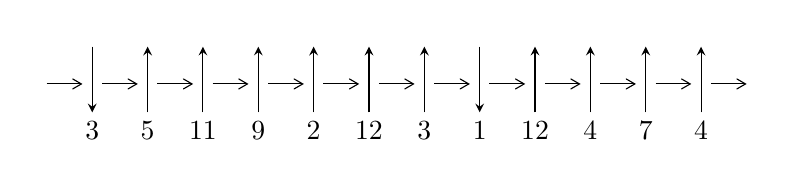
\begin{tikzpicture}[x=20pt, y=17pt]
	% nodes
	\node (C0) at (0, 0) {};
	\node (C1) at (1, 0) {};
	\node (C1U) at (1, +1) {};
	\node (C1D) at (1, -1) {3};

	\node (C2) at (2, 0) {};
	\node (C2U) at (2, +1) {};
	\node (C2D) at (2, -1) {5};

	\node (C3) at (3, 0) {};
	\node (C3U) at (3, +1) {};
	\node (C3D) at (3, -1) {11};

	\node (C4) at (4, 0) {};
	\node (C4U) at (4, +1) {};
	\node (C4D) at (4, -1) {9};

	\node (C5) at (5, 0) {};
	\node (C5U) at (5, +1) {};
	\node (C5D) at (5, -1) {2};

	\node (C6) at (6, 0) {};
	\node (C6U) at (6, +1) {};
	\node (C6D) at (6, -1) {12};

	\node (C7) at (7, 0) {};
	\node (C7U) at (7, +1) {};
	\node (C7D) at (7, -1) {3};

	\node (C8) at (8, 0) {};
	\node (C8U) at (8, +1) {};
	\node (C8D) at (8, -1) {1};

	\node (C9) at (9, 0) {};
	\node (C9U) at (9, +1) {};
	\node (C9D) at (9, -1) {12};

	\node (C10) at (10, 0) {};
	\node (C10U) at (10, +1) {};
	\node (C10D) at (10, -1) {4};

	\node (C11) at (11, 0) {};
	\node (C11U) at (11, +1) {};
	\node (C11D) at (11, -1) {7};

	\node (C12) at (12, 0) {};
	\node (C12U) at (12, +1) {};
	\node (C12D) at (12, -1) {4};
	\node (C13) at (13, 0) {};

	% arrows
	\draw[->,>={angle 60}]
	(C0) edge (C1) (C1) edge (C2) (C2) edge (C3) (C3) edge (C4) (C4) edge (C5) (C5) edge (C6) (C6) edge (C7) (C7) edge (C8) (C8) edge (C9) (C9) edge (C10) (C10) edge (C11) (C11) edge (C12) (C12) edge (C13) ;	\draw[->,>=stealth]
	(C1U) edge (C1D) (C2D) edge (C2U) (C3D) edge (C3U) (C4D) edge (C4U) (C5D) edge (C5U) (C6D) edge (C6U) (C7D) edge (C7U) (C8U) edge (C8D) (C9D) edge (C9U) (C10D) edge (C10U) (C11D) edge (C11U) (C12D) edge (C12U) ;
	\end{tikzpicture} \\
\hhline{~~} \\& 
\textbf{Solving Sequence} \\ \cline{2-2} 
 &
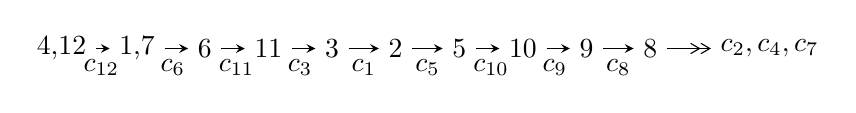
\begin{tikzpicture}[x=23pt, y=7pt]
	% node
	\node (A0) at (-1/8, 0) {4,12};
	\node (A1) at (17/16, 0) {1,7};
	\node (A2) at (17/8, 0) {6};
	\node (A3) at (25/8, 0) {11};
	\node (A4) at (33/8, 0) {3};
	\node (A5) at (41/8, 0) {2};
	\node (A6) at (49/8, 0) {5};
	\node (A7) at (57/8, 0) {10};
	\node (A8) at (65/8, 0) {9};
	\node (A9) at (73/8, 0) {8};
	\node (C1) at (1/2, -1) {$c_{12}$};
	\node (C2) at (13/8, -1) {$c_{6}$};
	\node (C3) at (21/8, -1) {$c_{11}$};
	\node (C4) at (29/8, -1) {$c_{3}$};
	\node (C5) at (37/8, -1) {$c_{1}$};
	\node (C6) at (45/8, -1) {$c_{5}$};
	\node (C7) at (53/8, -1) {$c_{10}$};
	\node (C8) at (61/8, -1) {$c_{9}$};
	\node (C9) at (69/8, -1) {$c_{8}$};
	\node (A10) at (11, 0) {$c_{2},c_{4},c_{7}$};

	% edge
	\draw[->,>=stealth]	
	(A0) edge (A1) (A1) edge (A2) (A2) edge (A3) (A3) edge (A4) (A4) edge (A5) (A5) edge (A6) (A6) edge (A7) (A7) edge (A8) (A8) edge (A9) ;
	\draw[->>,>={angle 60}]	
	(A9) edge (A10);
\end{tikzpicture} \\ 

\end{tabular} \\

\footnotetext{
The image of knot diagram is generated by the software ``\textbf{Draw programme}" developed by Andrew Bartholomew(\url{http://www.layer8.co.uk/maths/draw/index.htm\#Running-draw}), where we modified some parts for our purpose(\url{https://github.com/CATsTAILs/LinksPainter}).
}\phantom \\ \newline 
\centering \textbf{Ideals for irreducible components\footnotemark of $X_{\text{par}}$} 
 
\begin{align*}
I^u_{1}&=\langle 
-377702541 u^{18}-368786459 u^{17}+\cdots+156030809 b+1065050773,\\
\phantom{I^u_{1}}&\phantom{= \langle  }509610922 u^{18}+379813420 u^{17}+\cdots+156030809 a-1049301116,\;u^{19}+u^{18}+\cdots-3 u-1\rangle \\
I^u_{2}&=\langle 
1.29506\times10^{87} u^{39}+1.53497\times10^{87} u^{38}+\cdots+2.69800\times10^{88} b-3.45877\times10^{88},\\
\phantom{I^u_{2}}&\phantom{= \langle  }5.34951\times10^{86} u^{39}+5.15111\times10^{86} u^{38}+\cdots+2.69800\times10^{88} a+9.82066\times10^{88},\;u^{40}+u^{39}+\cdots-15 u+1\rangle \\
I^u_{3}&=\langle 
- u^{10}+29 u^9+25 u^8-45 u^7+31 u^6+58 u^5-50 u^4+86 u^3+101 u^2+47 b-20 u-11,\\
\phantom{I^u_{3}}&\phantom{= \langle  }31 u^{10}+41 u^9-23 u^8-15 u^7+26 u^6+35 u^5+93 u^4+60 u^3+65 u^2+47 a-38 u-129,\\
\phantom{I^u_{3}}&\phantom{= \langle  }u^{11}+u^{10}-2 u^9+3 u^7- u^6+2 u^5+4 u^4-2 u^3-2 u^2+1\rangle \\
I^u_{4}&=\langle 
-2 u^9+u^8+8 u^7+2 u^6-15 u^5-7 u^4+10 u^3+6 u^2+b-6 u-3,\\
\phantom{I^u_{4}}&\phantom{= \langle  }- u^9- u^8+6 u^7+5 u^6-10 u^5-11 u^4+8 u^3+8 u^2+a-5 u-6,\\
\phantom{I^u_{4}}&\phantom{= \langle  }u^{10}-4 u^8-3 u^7+6 u^6+7 u^5-2 u^4-5 u^3+u^2+3 u+1\rangle \\
\\
\end{align*}
\raggedright * 4 irreducible components of $\dim_{\mathbb{C}}=0$, with total 80 representations.\\
\footnotetext{All coefficients of polynomials are rational numbers. But the coefficients are sometimes approximated in decimal forms when there is not enough margin.}
\newpage
\renewcommand{\arraystretch}{1}
\centering \section*{I. $I^u_{1}= \langle -3.78\times10^{8} u^{18}-3.69\times10^{8} u^{17}+\cdots+1.56\times10^{8} b+1.07\times10^{9},\;5.10\times10^{8} u^{18}+3.80\times10^{8} u^{17}+\cdots+1.56\times10^{8} a-1.05\times10^{9},\;u^{19}+u^{18}+\cdots-3 u-1 \rangle$}
\flushleft \textbf{(i) Arc colorings}\\
\begin{tabular}{m{7pt} m{180pt} m{7pt} m{180pt} }
\flushright $a_{4}=$&$\begin{pmatrix}0\\u\end{pmatrix}$ \\
\flushright $a_{12}=$&$\begin{pmatrix}1\\0\end{pmatrix}$ \\
\flushright $a_{1}=$&$\begin{pmatrix}1\\- u^2\end{pmatrix}$ \\
\flushright $a_{7}=$&$\begin{pmatrix}-3.26609 u^{18}-2.43422 u^{17}+\cdots+14.6633 u+6.72496\\2.42069 u^{18}+2.36355 u^{17}+\cdots-9.38422 u-6.82590\end{pmatrix}$ \\
\flushright $a_{6}=$&$\begin{pmatrix}-5.68678 u^{18}-4.79777 u^{17}+\cdots+24.0475 u+13.5509\\2.42069 u^{18}+2.36355 u^{17}+\cdots-9.38422 u-6.82590\end{pmatrix}$ \\
\flushright $a_{11}=$&$\begin{pmatrix}8.21607 u^{18}+4.60275 u^{17}+\cdots-30.9090 u-8.69525\\-0.467933 u^{18}-1.05048 u^{17}+\cdots+3.62390 u+3.61332\end{pmatrix}$ \\
\flushright $a_{3}=$&$\begin{pmatrix}2.94393 u^{18}+3.81230 u^{17}+\cdots-11.6400 u-13.6846\\0.852487 u^{18}-0.589367 u^{17}+\cdots-1.92514 u+2.74496\end{pmatrix}$ \\
\flushright $a_{2}=$&$\begin{pmatrix}4.03573 u^{18}+2.94704 u^{17}+\cdots-19.3471 u-5.85388\\-1.97347 u^{18}-0.834541 u^{17}+\cdots+6.74227 u+1.47324\end{pmatrix}$ \\
\flushright $a_{5}=$&$\begin{pmatrix}-3.87980 u^{18}-5.91327 u^{17}+\cdots+16.8878 u+20.9112\\0.467933 u^{18}+1.05048 u^{17}+\cdots-1.62390 u-3.61332\end{pmatrix}$ \\
\flushright $a_{10}=$&$\begin{pmatrix}8.21607 u^{18}+4.60275 u^{17}+\cdots-30.9090 u-8.69525\\u\end{pmatrix}$ \\
\flushright $a_{9}=$&$\begin{pmatrix}8.21607 u^{18}+4.60275 u^{17}+\cdots-31.9090 u-8.69525\\u\end{pmatrix}$ \\
\flushright $a_{8}=$&$\begin{pmatrix}8.68401 u^{18}+5.65323 u^{17}+\cdots-33.5329 u-12.3086\\0.580147 u^{18}+0.361879 u^{17}+\cdots-1.21559 u-0.582551\end{pmatrix}$\\&\end{tabular}
\flushleft \textbf{(ii) Obstruction class $= -1$}\\~\\
\flushleft \textbf{(iii) Cusp Shapes $= -\frac{858705183}{156030809} u^{18}-\frac{1012526591}{156030809} u^{17}+\cdots+\frac{5471923598}{156030809} u+\frac{4145235745}{156030809}$}\\~\\
\newpage\renewcommand{\arraystretch}{1}
\flushleft \textbf{(iv) u-Polynomials at the component}\newline \\
\begin{tabular}{m{50pt}|m{274pt}}
Crossings & \hspace{64pt}u-Polynomials at each crossing \\
\hline $$\begin{aligned}c_{1}\end{aligned}$$&$\begin{aligned}
&u^{19}+7 u^{18}+\cdots-4 u-1
\end{aligned}$\\
\hline $$\begin{aligned}c_{2},c_{5},c_{6}\\c_{11}\end{aligned}$$&$\begin{aligned}
&u^{19}+u^{18}+\cdots+2 u-1
\end{aligned}$\\
\hline $$\begin{aligned}c_{3},c_{10}\end{aligned}$$&$\begin{aligned}
&u^{19}-11 u^{18}+\cdots+60 u-8
\end{aligned}$\\
\hline $$\begin{aligned}c_{4}\end{aligned}$$&$\begin{aligned}
&u^{19}+12 u^{18}+\cdots-176 u-32
\end{aligned}$\\
\hline $$\begin{aligned}c_{7}\end{aligned}$$&$\begin{aligned}
&u^{19}- u^{18}+\cdots+1133 u-517
\end{aligned}$\\
\hline $$\begin{aligned}c_{8}\end{aligned}$$&$\begin{aligned}
&u^{19}+11 u^{17}+\cdots-7 u-13
\end{aligned}$\\
\hline $$\begin{aligned}c_{9},c_{12}\end{aligned}$$&$\begin{aligned}
&u^{19}+u^{18}+\cdots-3 u-1
\end{aligned}$\\
\hline
\end{tabular}\\~\\
\newpage\renewcommand{\arraystretch}{1}
\flushleft \textbf{(v) Riley Polynomials at the component}\newline \\
\begin{tabular}{m{50pt}|m{274pt}}
Crossings & \hspace{64pt}Riley Polynomials at each crossing \\
\hline $$\begin{aligned}c_{1}\end{aligned}$$&$\begin{aligned}
&y^{19}+23 y^{18}+\cdots+28 y-1
\end{aligned}$\\
\hline $$\begin{aligned}c_{2},c_{5},c_{6}\\c_{11}\end{aligned}$$&$\begin{aligned}
&y^{19}+7 y^{18}+\cdots-4 y-1
\end{aligned}$\\
\hline $$\begin{aligned}c_{3},c_{10}\end{aligned}$$&$\begin{aligned}
&y^{19}+3 y^{18}+\cdots-368 y-64
\end{aligned}$\\
\hline $$\begin{aligned}c_{4}\end{aligned}$$&$\begin{aligned}
&y^{19}+8 y^{18}+\cdots+6912 y-1024
\end{aligned}$\\
\hline $$\begin{aligned}c_{7}\end{aligned}$$&$\begin{aligned}
&y^{19}-7 y^{18}+\cdots+566093 y-267289
\end{aligned}$\\
\hline $$\begin{aligned}c_{8}\end{aligned}$$&$\begin{aligned}
&y^{19}+22 y^{18}+\cdots-2291 y-169
\end{aligned}$\\
\hline $$\begin{aligned}c_{9},c_{12}\end{aligned}$$&$\begin{aligned}
&y^{19}-23 y^{18}+\cdots+9 y-1
\end{aligned}$\\
\hline
\end{tabular}\\~\\
\newpage\flushleft \textbf{(vi) Complex Volumes and Cusp Shapes}
$$\begin{array}{c|c|c}  
\text{Solutions to }I^u_{1}& \I (\text{vol} + \sqrt{-1}CS) & \text{Cusp shape}\\
 \hline 
\begin{aligned}
u &= -1.043320 + 0.605021 I \\
a &= -0.095431 - 1.196260 I \\
b &= -0.072994 - 1.051030 I\end{aligned}
 & -3.46673 - 2.11998 I & \phantom{-}0.23396 + 2.61296 I \\ \hline\begin{aligned}
u &= -1.043320 - 0.605021 I \\
a &= -0.095431 + 1.196260 I \\
b &= -0.072994 + 1.051030 I\end{aligned}
 & -3.46673 + 2.11998 I & \phantom{-}0.23396 - 2.61296 I \\ \hline\begin{aligned}
u &= \phantom{-}1.279840 + 0.395378 I \\
a &= \phantom{-}0.190387 - 0.406271 I \\
b &= \phantom{-}0.221252 - 0.463223 I\end{aligned}
 & \phantom{-}1.07628 + 1.45118 I & \phantom{-}13.08253 + 0.58489 I \\ \hline\begin{aligned}
u &= \phantom{-}1.279840 - 0.395378 I \\
a &= \phantom{-}0.190387 + 0.406271 I \\
b &= \phantom{-}0.221252 + 0.463223 I\end{aligned}
 & \phantom{-}1.07628 - 1.45118 I & \phantom{-}13.08253 - 0.58489 I \\ \hline\begin{aligned}
u &= -0.091308 + 0.542033 I \\
a &= -0.05772 - 3.40851 I \\
b &= -0.321625 - 0.991324 I\end{aligned}
 & -6.77802 + 4.24933 I & -2.37252 - 3.20470 I \\ \hline\begin{aligned}
u &= -0.091308 - 0.542033 I \\
a &= -0.05772 + 3.40851 I \\
b &= -0.321625 + 0.991324 I\end{aligned}
 & -6.77802 - 4.24933 I & -2.37252 + 3.20470 I \\ \hline\begin{aligned}
u &= -0.396664 + 0.369740 I \\
a &= \phantom{-}1.23276 + 1.31882 I \\
b &= \phantom{-}0.190738 + 0.915706 I\end{aligned}
 & -2.12350 + 1.85148 I & \phantom{-}4.32931 - 4.24457 I \\ \hline\begin{aligned}
u &= -0.396664 - 0.369740 I \\
a &= \phantom{-}1.23276 - 1.31882 I \\
b &= \phantom{-}0.190738 - 0.915706 I\end{aligned}
 & -2.12350 - 1.85148 I & \phantom{-}4.32931 + 4.24457 I \\ \hline\begin{aligned}
u &= \phantom{-}1.49967 + 0.06625 I \\
a &= -0.574936 - 0.248373 I \\
b &= \phantom{-}0.819301 + 1.051500 I\end{aligned}
 & \phantom{-}8.33063 + 6.97397 I & \phantom{-}8.76530 - 4.76080 I \\ \hline\begin{aligned}
u &= \phantom{-}1.49967 - 0.06625 I \\
a &= -0.574936 + 0.248373 I \\
b &= \phantom{-}0.819301 - 1.051500 I\end{aligned}
 & \phantom{-}8.33063 - 6.97397 I & \phantom{-}8.76530 + 4.76080 I\\
 \hline 
 \end{array}$$\newpage$$\begin{array}{c|c|c}  
\text{Solutions to }I^u_{1}& \I (\text{vol} + \sqrt{-1}CS) & \text{Cusp shape}\\
 \hline 
\begin{aligned}
u &= -0.356851 + 0.335765 I \\
a &= \phantom{-}1.25082 + 2.28548 I \\
b &= -0.656301 - 0.536511 I\end{aligned}
 & -3.49379 + 2.71619 I & \phantom{-}7.39466 - 0.32501 I \\ \hline\begin{aligned}
u &= -0.356851 - 0.335765 I \\
a &= \phantom{-}1.25082 - 2.28548 I \\
b &= -0.656301 + 0.536511 I\end{aligned}
 & -3.49379 - 2.71619 I & \phantom{-}7.39466 + 0.32501 I \\ \hline\begin{aligned}
u &= -1.56268 + 0.05774 I \\
a &= -1.259550 - 0.485799 I \\
b &= \phantom{-}0.975642 - 0.970457 I\end{aligned}
 & \phantom{-}9.19399 - 6.70093 I & \phantom{-}9.82122 + 4.48583 I \\ \hline\begin{aligned}
u &= -1.56268 - 0.05774 I \\
a &= -1.259550 + 0.485799 I \\
b &= \phantom{-}0.975642 + 0.970457 I\end{aligned}
 & \phantom{-}9.19399 + 6.70093 I & \phantom{-}9.82122 - 4.48583 I \\ \hline\begin{aligned}
u &= \phantom{-}0.315741\phantom{ +0.000000I} \\
a &= \phantom{-}1.20666\phantom{ +0.000000I} \\
b &= \phantom{-}0.408538\phantom{ +0.000000I}\end{aligned}
 & \phantom{-}0.727380\phantom{ +0.000000I} & \phantom{-}13.8820\phantom{ +0.000000I} \\ \hline\begin{aligned}
u &= \phantom{-}1.68314 + 0.54519 I \\
a &= \phantom{-}0.259507 - 0.084155 I \\
b &= -0.986094 + 0.888888 I\end{aligned}
 & \phantom{-}9.98818 + 1.53259 I & \phantom{-}10.28519 + 0.05847 I \\ \hline\begin{aligned}
u &= \phantom{-}1.68314 - 0.54519 I \\
a &= \phantom{-}0.259507 + 0.084155 I \\
b &= -0.986094 - 0.888888 I\end{aligned}
 & \phantom{-}9.98818 - 1.53259 I & \phantom{-}10.28519 - 0.05847 I \\ \hline\begin{aligned}
u &= -1.66969 + 0.71456 I \\
a &= \phantom{-}0.950831 + 0.876319 I \\
b &= -0.87419 + 1.14110 I\end{aligned}
 & \phantom{-}8.2934 - 15.6503 I & \phantom{-}8.00000 + 8.25494 I \\ \hline\begin{aligned}
u &= -1.66969 - 0.71456 I \\
a &= \phantom{-}0.950831 - 0.876319 I \\
b &= -0.87419 - 1.14110 I\end{aligned}
 & \phantom{-}8.2934 + 15.6503 I & \phantom{-}8.00000 - 8.25494 I\\
 \hline 
 \end{array}$$\newpage\newpage\renewcommand{\arraystretch}{1}
\centering \section*{II. $I^u_{2}= \langle 1.30\times10^{87} u^{39}+1.53\times10^{87} u^{38}+\cdots+2.70\times10^{88} b-3.46\times10^{88},\;5.35\times10^{86} u^{39}+5.15\times10^{86} u^{38}+\cdots+2.70\times10^{88} a+9.82\times10^{88},\;u^{40}+u^{39}+\cdots-15 u+1 \rangle$}
\flushleft \textbf{(i) Arc colorings}\\
\begin{tabular}{m{7pt} m{180pt} m{7pt} m{180pt} }
\flushright $a_{4}=$&$\begin{pmatrix}0\\u\end{pmatrix}$ \\
\flushright $a_{12}=$&$\begin{pmatrix}1\\0\end{pmatrix}$ \\
\flushright $a_{1}=$&$\begin{pmatrix}1\\- u^2\end{pmatrix}$ \\
\flushright $a_{7}=$&$\begin{pmatrix}-0.0198277 u^{39}-0.0190923 u^{38}+\cdots-44.7904 u-3.63997\\-0.0480005 u^{39}-0.0568927 u^{38}+\cdots+0.311946 u+1.28197\end{pmatrix}$ \\
\flushright $a_{6}=$&$\begin{pmatrix}0.0281728 u^{39}+0.0378004 u^{38}+\cdots-45.1024 u-4.92194\\-0.0480005 u^{39}-0.0568927 u^{38}+\cdots+0.311946 u+1.28197\end{pmatrix}$ \\
\flushright $a_{11}=$&$\begin{pmatrix}0.536629 u^{39}+0.596877 u^{38}+\cdots-25.4262 u-5.72637\\-0.0756455 u^{39}-0.0881317 u^{38}+\cdots+1.50300 u+0.486117\end{pmatrix}$ \\
\flushright $a_{3}=$&$\begin{pmatrix}0.458136 u^{39}+0.471790 u^{38}+\cdots+63.8377 u-7.67485\\-0.0990701 u^{39}-0.0884537 u^{38}+\cdots-17.1405 u+0.775723\end{pmatrix}$ \\
\flushright $a_{2}=$&$\begin{pmatrix}0.0573134 u^{39}+0.0688277 u^{38}+\cdots+43.4630 u+6.53740\\0.0953537 u^{39}+0.101112 u^{38}+\cdots+5.88241 u-2.22024\end{pmatrix}$ \\
\flushright $a_{5}=$&$\begin{pmatrix}-0.638325 u^{39}-0.657958 u^{38}+\cdots-103.579 u+9.05298\\0.0880767 u^{39}+0.0956592 u^{38}+\cdots+22.3476 u-0.616054\end{pmatrix}$ \\
\flushright $a_{10}=$&$\begin{pmatrix}0.536629 u^{39}+0.596877 u^{38}+\cdots-25.4262 u-5.72637\\-0.0734017 u^{39}-0.0888770 u^{38}+\cdots+1.87009 u+0.425868\end{pmatrix}$ \\
\flushright $a_{9}=$&$\begin{pmatrix}0.610031 u^{39}+0.685754 u^{38}+\cdots-27.2963 u-6.15224\\-0.0734017 u^{39}-0.0888770 u^{38}+\cdots+1.87009 u+0.425868\end{pmatrix}$ \\
\flushright $a_{8}=$&$\begin{pmatrix}0.542040 u^{39}+0.596575 u^{38}+\cdots-24.9003 u-5.80209\\-0.0788525 u^{39}-0.0842106 u^{38}+\cdots+2.11993 u+0.404680\end{pmatrix}$\\&\end{tabular}
\flushleft \textbf{(ii) Obstruction class $= -1$}\\~\\
\flushleft \textbf{(iii) Cusp Shapes $= 0.442497 u^{39}+0.473863 u^{38}+\cdots+3.13307 u+13.3769$}\\~\\
\newpage\renewcommand{\arraystretch}{1}
\flushleft \textbf{(iv) u-Polynomials at the component}\newline \\
\begin{tabular}{m{50pt}|m{274pt}}
Crossings & \hspace{64pt}u-Polynomials at each crossing \\
\hline $$\begin{aligned}c_{1}\end{aligned}$$&$\begin{aligned}
&u^{40}+8 u^{39}+\cdots+1381 u+121
\end{aligned}$\\
\hline $$\begin{aligned}c_{2},c_{5},c_{6}\\c_{11}\end{aligned}$$&$\begin{aligned}
&u^{40}-2 u^{39}+\cdots+29 u+11
\end{aligned}$\\
\hline $$\begin{aligned}c_{3},c_{10}\end{aligned}$$&$\begin{aligned}
&(u^{20}+5 u^{19}+\cdots+5 u+1)^{2}
\end{aligned}$\\
\hline $$\begin{aligned}c_{4}\end{aligned}$$&$\begin{aligned}
&(u^{20}-5 u^{19}+\cdots-6 u+1)^{2}
\end{aligned}$\\
\hline $$\begin{aligned}c_{7}\end{aligned}$$&$\begin{aligned}
&u^{40}-18 u^{38}+\cdots+26588 u+210103
\end{aligned}$\\
\hline $$\begin{aligned}c_{8}\end{aligned}$$&$\begin{aligned}
&u^{40}-2 u^{39}+\cdots-350134 u+28487
\end{aligned}$\\
\hline $$\begin{aligned}c_{9},c_{12}\end{aligned}$$&$\begin{aligned}
&u^{40}+u^{39}+\cdots-15 u+1
\end{aligned}$\\
\hline
\end{tabular}\\~\\
\newpage\renewcommand{\arraystretch}{1}
\flushleft \textbf{(v) Riley Polynomials at the component}\newline \\
\begin{tabular}{m{50pt}|m{274pt}}
Crossings & \hspace{64pt}Riley Polynomials at each crossing \\
\hline $$\begin{aligned}c_{1}\end{aligned}$$&$\begin{aligned}
&y^{40}+40 y^{39}+\cdots+111361 y+14641
\end{aligned}$\\
\hline $$\begin{aligned}c_{2},c_{5},c_{6}\\c_{11}\end{aligned}$$&$\begin{aligned}
&y^{40}+8 y^{39}+\cdots+1381 y+121
\end{aligned}$\\
\hline $$\begin{aligned}c_{3},c_{10}\end{aligned}$$&$\begin{aligned}
&(y^{20}- y^{19}+\cdots-9 y+1)^{2}
\end{aligned}$\\
\hline $$\begin{aligned}c_{4}\end{aligned}$$&$\begin{aligned}
&(y^{20}- y^{19}+\cdots-20 y+1)^{2}
\end{aligned}$\\
\hline $$\begin{aligned}c_{7}\end{aligned}$$&$\begin{aligned}
&y^{40}-36 y^{39}+\cdots+252213388832 y+44143270609
\end{aligned}$\\
\hline $$\begin{aligned}c_{8}\end{aligned}$$&$\begin{aligned}
&y^{40}+40 y^{39}+\cdots-4553546458 y+811509169
\end{aligned}$\\
\hline $$\begin{aligned}c_{9},c_{12}\end{aligned}$$&$\begin{aligned}
&y^{40}-33 y^{39}+\cdots+5 y+1
\end{aligned}$\\
\hline
\end{tabular}\\~\\
\newpage\flushleft \textbf{(vi) Complex Volumes and Cusp Shapes}
$$\begin{array}{c|c|c}  
\text{Solutions to }I^u_{2}& \I (\text{vol} + \sqrt{-1}CS) & \text{Cusp shape}\\
 \hline 
\begin{aligned}
u &= \phantom{-}0.789817 + 0.551198 I \\
a &= -0.69551 + 1.55288 I \\
b &= \phantom{-}0.459315 + 1.209800 I\end{aligned}
 & -1.25686 + 2.87744 I & \phantom{-}8.53861 + 0.21509 I \\ \hline\begin{aligned}
u &= \phantom{-}0.789817 - 0.551198 I \\
a &= -0.69551 - 1.55288 I \\
b &= \phantom{-}0.459315 - 1.209800 I\end{aligned}
 & -1.25686 - 2.87744 I & \phantom{-}8.53861 - 0.21509 I \\ \hline\begin{aligned}
u &= -0.882283 + 0.194843 I \\
a &= -0.417404 - 0.174483 I \\
b &= \phantom{-}1.234230 + 0.246821 I\end{aligned}
 & \phantom{-}3.22335 - 0.66671 I & \phantom{-}5.55879 + 11.26225 I \\ \hline\begin{aligned}
u &= -0.882283 - 0.194843 I \\
a &= -0.417404 + 0.174483 I \\
b &= \phantom{-}1.234230 - 0.246821 I\end{aligned}
 & \phantom{-}3.22335 + 0.66671 I & \phantom{-}5.55879 - 11.26225 I \\ \hline\begin{aligned}
u &= \phantom{-}1.096700 + 0.080097 I \\
a &= -0.169582 - 0.382784 I \\
b &= \phantom{-}0.661294 + 0.316017 I\end{aligned}
 & \phantom{-}1.73797 + 1.66833 I & \phantom{-}9.09788 - 4.11752 I \\ \hline\begin{aligned}
u &= \phantom{-}1.096700 - 0.080097 I \\
a &= -0.169582 + 0.382784 I \\
b &= \phantom{-}0.661294 - 0.316017 I\end{aligned}
 & \phantom{-}1.73797 - 1.66833 I & \phantom{-}9.09788 + 4.11752 I \\ \hline\begin{aligned}
u &= -0.702136 + 0.452232 I \\
a &= \phantom{-}1.65697 + 0.89964 I \\
b &= -0.604929 + 1.075710 I\end{aligned}
 & -5.01038 - 2.16864 I & \phantom{-}2.33481 + 6.10094 I \\ \hline\begin{aligned}
u &= -0.702136 - 0.452232 I \\
a &= \phantom{-}1.65697 - 0.89964 I \\
b &= -0.604929 - 1.075710 I\end{aligned}
 & -5.01038 + 2.16864 I & \phantom{-}2.33481 - 6.10094 I \\ \hline\begin{aligned}
u &= -1.178690 + 0.159087 I \\
a &= \phantom{-}0.183886 + 0.503919 I \\
b &= -0.538174 + 0.434982 I\end{aligned}
 & -0.69886 - 4.77224 I & \phantom{-}8.00000 + 7.57794 I \\ \hline\begin{aligned}
u &= -1.178690 - 0.159087 I \\
a &= \phantom{-}0.183886 - 0.503919 I \\
b &= -0.538174 - 0.434982 I\end{aligned}
 & -0.69886 + 4.77224 I & \phantom{-}8.00000 - 7.57794 I\\
 \hline 
 \end{array}$$\newpage$$\begin{array}{c|c|c}  
\text{Solutions to }I^u_{2}& \I (\text{vol} + \sqrt{-1}CS) & \text{Cusp shape}\\
 \hline 
\begin{aligned}
u &= -1.000670 + 0.723305 I \\
a &= -0.588918 - 1.139490 I \\
b &= \phantom{-}0.40494 - 1.37467 I\end{aligned}
 & -1.08479 - 6.65241 I & \phantom{-}8.00000 + 8.68586 I \\ \hline\begin{aligned}
u &= -1.000670 - 0.723305 I \\
a &= -0.588918 + 1.139490 I \\
b &= \phantom{-}0.40494 + 1.37467 I\end{aligned}
 & -1.08479 + 6.65241 I & \phantom{-}8.00000 - 8.68586 I \\ \hline\begin{aligned}
u &= \phantom{-}0.958749 + 0.984714 I \\
a &= -0.41472 + 1.38571 I \\
b &= \phantom{-}0.465289 + 0.991245 I\end{aligned}
 & -0.69886 + 4.77224 I & \phantom{-0.000000 } 0 \\ \hline\begin{aligned}
u &= \phantom{-}0.958749 - 0.984714 I \\
a &= -0.41472 - 1.38571 I \\
b &= \phantom{-}0.465289 - 0.991245 I\end{aligned}
 & -0.69886 - 4.77224 I & \phantom{-0.000000 } 0 \\ \hline\begin{aligned}
u &= -1.50241 + 0.07716 I \\
a &= -0.496444 - 0.235822 I \\
b &= \phantom{-}0.983741 + 0.983994 I\end{aligned}
 & \phantom{-}9.17040 + 0.45837 I & \phantom{-0.000000 } 0 \\ \hline\begin{aligned}
u &= -1.50241 - 0.07716 I \\
a &= -0.496444 + 0.235822 I \\
b &= \phantom{-}0.983741 - 0.983994 I\end{aligned}
 & \phantom{-}9.17040 - 0.45837 I & \phantom{-0.000000 } 0 \\ \hline\begin{aligned}
u &= \phantom{-}1.50669 + 0.14155 I \\
a &= -1.44000 - 0.34489 I \\
b &= \phantom{-}0.940968 - 0.791711 I\end{aligned}
 & \phantom{-}9.17040 + 0.45837 I & \phantom{-0.000000 } 0 \\ \hline\begin{aligned}
u &= \phantom{-}1.50669 - 0.14155 I \\
a &= -1.44000 + 0.34489 I \\
b &= \phantom{-}0.940968 + 0.791711 I\end{aligned}
 & \phantom{-}9.17040 - 0.45837 I & \phantom{-0.000000 } 0 \\ \hline\begin{aligned}
u &= -1.52444 + 0.02714 I \\
a &= \phantom{-}0.708019 + 0.222574 I \\
b &= -0.352756 + 0.830770 I\end{aligned}
 & -1.25686 + 2.87744 I & \phantom{-0.000000 } 0 \\ \hline\begin{aligned}
u &= -1.52444 - 0.02714 I \\
a &= \phantom{-}0.708019 - 0.222574 I \\
b &= -0.352756 - 0.830770 I\end{aligned}
 & -1.25686 - 2.87744 I & \phantom{-0.000000 } 0\\
 \hline 
 \end{array}$$\newpage$$\begin{array}{c|c|c}  
\text{Solutions to }I^u_{2}& \I (\text{vol} + \sqrt{-1}CS) & \text{Cusp shape}\\
 \hline 
\begin{aligned}
u &= -0.284736 + 0.328185 I \\
a &= -4.60209 - 1.08232 I \\
b &= -0.118953 + 0.502474 I\end{aligned}
 & -5.01038 + 2.16864 I & \phantom{-}2.33481 - 6.10094 I \\ \hline\begin{aligned}
u &= -0.284736 - 0.328185 I \\
a &= -4.60209 + 1.08232 I \\
b &= -0.118953 - 0.502474 I\end{aligned}
 & -5.01038 - 2.16864 I & \phantom{-}2.33481 + 6.10094 I \\ \hline\begin{aligned}
u &= \phantom{-}1.59822 + 0.22825 I \\
a &= \phantom{-}0.335646 - 0.321778 I \\
b &= -0.129954 - 0.886577 I\end{aligned}
 & \phantom{-}1.73797 + 1.66833 I & \phantom{-0.000000 } 0 \\ \hline\begin{aligned}
u &= \phantom{-}1.59822 - 0.22825 I \\
a &= \phantom{-}0.335646 + 0.321778 I \\
b &= -0.129954 + 0.886577 I\end{aligned}
 & \phantom{-}1.73797 - 1.66833 I & \phantom{-0.000000 } 0 \\ \hline\begin{aligned}
u &= -1.60666 + 0.21833 I \\
a &= \phantom{-}1.27939 + 0.87709 I \\
b &= -0.562169 + 0.793968 I\end{aligned}
 & -1.08479 - 6.65241 I & \phantom{-0.000000 } 0 \\ \hline\begin{aligned}
u &= -1.60666 - 0.21833 I \\
a &= \phantom{-}1.27939 - 0.87709 I \\
b &= -0.562169 - 0.793968 I\end{aligned}
 & -1.08479 + 6.65241 I & \phantom{-0.000000 } 0 \\ \hline\begin{aligned}
u &= -1.56979 + 0.64601 I \\
a &= \phantom{-}0.224170 + 0.117637 I \\
b &= -1.115240 - 0.763070 I\end{aligned}
 & \phantom{-}9.55391 - 8.46488 I & \phantom{-0.000000 } 0 \\ \hline\begin{aligned}
u &= -1.56979 - 0.64601 I \\
a &= \phantom{-}0.224170 - 0.117637 I \\
b &= -1.115240 + 0.763070 I\end{aligned}
 & \phantom{-}9.55391 + 8.46488 I & \phantom{-0.000000 } 0 \\ \hline\begin{aligned}
u &= \phantom{-}1.74383 + 0.19203 I \\
a &= \phantom{-}1.44796 + 1.25852 I \\
b &= -0.391026 + 0.507425 I\end{aligned}
 & \phantom{-}3.22335 - 0.66671 I & \phantom{-0.000000 } 0 \\ \hline\begin{aligned}
u &= \phantom{-}1.74383 - 0.19203 I \\
a &= \phantom{-}1.44796 - 1.25852 I \\
b &= -0.391026 - 0.507425 I\end{aligned}
 & \phantom{-}3.22335 + 0.66671 I & \phantom{-0.000000 } 0\\
 \hline 
 \end{array}$$\newpage$$\begin{array}{c|c|c}  
\text{Solutions to }I^u_{2}& \I (\text{vol} + \sqrt{-1}CS) & \text{Cusp shape}\\
 \hline 
\begin{aligned}
u &= \phantom{-}0.46290 + 1.79705 I \\
a &= \phantom{-}0.361971 + 0.723514 I \\
b &= -0.776259 + 0.727271 I\end{aligned}
 & \phantom{-}3.67864 + 0.89894 I & \phantom{-0.000000 } 0 \\ \hline\begin{aligned}
u &= \phantom{-}0.46290 - 1.79705 I \\
a &= \phantom{-}0.361971 - 0.723514 I \\
b &= -0.776259 - 0.727271 I\end{aligned}
 & \phantom{-}3.67864 - 0.89894 I & \phantom{-0.000000 } 0 \\ \hline\begin{aligned}
u &= \phantom{-}1.76739 + 0.61988 I \\
a &= \phantom{-}1.022920 - 0.802923 I \\
b &= -0.906801 - 1.018680 I\end{aligned}
 & \phantom{-}9.55391 + 8.46488 I & \phantom{-0.000000 } 0 \\ \hline\begin{aligned}
u &= \phantom{-}1.76739 - 0.61988 I \\
a &= \phantom{-}1.022920 + 0.802923 I \\
b &= -0.906801 + 1.018680 I\end{aligned}
 & \phantom{-}9.55391 - 8.46488 I & \phantom{-0.000000 } 0 \\ \hline\begin{aligned}
u &= -0.0113205 + 0.0913606 I \\
a &= -2.90917 - 4.34403 I \\
b &= \phantom{-}1.072060 + 0.812581 I\end{aligned}
 & \phantom{-}3.67864 + 0.89894 I & \phantom{-}14.7379 - 6.8397 I \\ \hline\begin{aligned}
u &= -0.0113205 - 0.0913606 I \\
a &= -2.90917 + 4.34403 I \\
b &= \phantom{-}1.072060 - 0.812581 I\end{aligned}
 & \phantom{-}3.67864 - 0.89894 I & \phantom{-}14.7379 + 6.8397 I \\ \hline\begin{aligned}
u &= \phantom{-}0.0698929 + 0.0329543 I \\
a &= -6.77015 - 1.38688 I \\
b &= \phantom{-}0.98494 - 1.07091 I\end{aligned}
 & \phantom{-}2.89322 - 6.53100 I & \phantom{-}16.6269 + 9.9012 I \\ \hline\begin{aligned}
u &= \phantom{-}0.0698929 - 0.0329543 I \\
a &= -6.77015 + 1.38688 I \\
b &= \phantom{-}0.98494 + 1.07091 I\end{aligned}
 & \phantom{-}2.89322 + 6.53100 I & \phantom{-}16.6269 - 9.9012 I \\ \hline\begin{aligned}
u &= -0.23102 + 2.12015 I \\
a &= \phantom{-}0.283053 - 0.859606 I \\
b &= -0.710501 - 0.983550 I\end{aligned}
 & \phantom{-}2.89322 + 6.53100 I & \phantom{-0.000000 } 0 \\ \hline\begin{aligned}
u &= -0.23102 - 2.12015 I \\
a &= \phantom{-}0.283053 + 0.859606 I \\
b &= -0.710501 + 0.983550 I\end{aligned}
 & \phantom{-}2.89322 - 6.53100 I & \phantom{-0.000000 } 0\\
 \hline 
 \end{array}$$\newpage\newpage\renewcommand{\arraystretch}{1}
\centering \section*{III. $I^u_{3}= \langle - u^{10}+29 u^9+\cdots+47 b-11,\;31 u^{10}+41 u^9+\cdots+47 a-129,\;u^{11}+u^{10}+\cdots-2 u^2+1 \rangle$}
\flushleft \textbf{(i) Arc colorings}\\
\begin{tabular}{m{7pt} m{180pt} m{7pt} m{180pt} }
\flushright $a_{4}=$&$\begin{pmatrix}0\\u\end{pmatrix}$ \\
\flushright $a_{12}=$&$\begin{pmatrix}1\\0\end{pmatrix}$ \\
\flushright $a_{1}=$&$\begin{pmatrix}1\\- u^2\end{pmatrix}$ \\
\flushright $a_{7}=$&$\begin{pmatrix}-0.659574 u^{10}-0.872340 u^{9}+\cdots+0.808511 u+2.74468\\0.0212766 u^{10}-0.617021 u^{9}+\cdots+0.425532 u+0.234043\end{pmatrix}$ \\
\flushright $a_{6}=$&$\begin{pmatrix}-0.680851 u^{10}-0.255319 u^{9}+\cdots+0.382979 u+2.51064\\0.0212766 u^{10}-0.617021 u^{9}+\cdots+0.425532 u+0.234043\end{pmatrix}$ \\
\flushright $a_{11}=$&$\begin{pmatrix}-0.170213 u^{10}-1.06383 u^{9}+\cdots+0.595745 u+0.127660\\0.191489 u^{10}+0.446809 u^{9}+\cdots-1.17021 u-0.893617\end{pmatrix}$ \\
\flushright $a_{3}=$&$\begin{pmatrix}-2.04255 u^{10}-2.76596 u^{9}+\cdots+4.14894 u+1.53191\\0.106383 u^{10}-0.0851064 u^{9}+\cdots-0.872340 u+0.170213\end{pmatrix}$ \\
\flushright $a_{2}=$&$\begin{pmatrix}-2.17021 u^{10}-3.06383 u^{9}+\cdots+0.595745 u+3.12766\\0.744681 u^{10}+0.404255 u^{9}+\cdots-1.10638 u-0.808511\end{pmatrix}$ \\
\flushright $a_{5}=$&$\begin{pmatrix}1.65957 u^{10}+1.87234 u^{9}+\cdots-3.80851 u+0.255319\\0.191489 u^{10}+0.446809 u^{9}+\cdots+0.829787 u-0.893617\end{pmatrix}$ \\
\flushright $a_{10}=$&$\begin{pmatrix}-0.170213 u^{10}-1.06383 u^{9}+\cdots+0.595745 u+0.127660\\- u\end{pmatrix}$ \\
\flushright $a_{9}=$&$\begin{pmatrix}-0.170213 u^{10}-1.06383 u^{9}+\cdots+1.59574 u+0.127660\\- u\end{pmatrix}$ \\
\flushright $a_{8}=$&$\begin{pmatrix}-0.361702 u^{10}-1.51064 u^{9}+\cdots+0.765957 u+1.02128\\0.340426 u^{10}+0.127660 u^{9}+\cdots-1.19149 u-0.255319\end{pmatrix}$\\&\end{tabular}
\flushleft \textbf{(ii) Obstruction class $= 1$}\\~\\
\flushleft \textbf{(iii) Cusp Shapes $= \frac{69}{47} u^{10}-\frac{168}{47} u^9-\frac{315}{47} u^8+\frac{379}{47} u^7+\frac{117}{47} u^6-\frac{524}{47} u^5+\frac{254}{47} u^4-\frac{388}{47} u^3-\frac{906}{47} u^2+\frac{111}{47} u+\frac{524}{47}$}\\~\\
\newpage\renewcommand{\arraystretch}{1}
\flushleft \textbf{(iv) u-Polynomials at the component}\newline \\
\begin{tabular}{m{50pt}|m{274pt}}
Crossings & \hspace{64pt}u-Polynomials at each crossing \\
\hline $$\begin{aligned}c_{1}\end{aligned}$$&$\begin{aligned}
&u^{11}-5 u^{10}+\cdots-5 u+1
\end{aligned}$\\
\hline $$\begin{aligned}c_{2},c_{6}\end{aligned}$$&$\begin{aligned}
&u^{11}+u^{10}+3 u^9+2 u^8+5 u^7+3 u^6+5 u^5+3 u^4+3 u^3+3 u^2+u+1
\end{aligned}$\\
\hline $$\begin{aligned}c_{3}\end{aligned}$$&$\begin{aligned}
&u^{11}-4 u^{10}+\cdots+u-1
\end{aligned}$\\
\hline $$\begin{aligned}c_{4}\end{aligned}$$&$\begin{aligned}
&u^{11}+u^{10}+5 u^9+4 u^8+7 u^7+4 u^6+u^5+u^4-2 u^3+2 u^2+1
\end{aligned}$\\
\hline $$\begin{aligned}c_{5},c_{11}\end{aligned}$$&$\begin{aligned}
&u^{11}- u^{10}+3 u^9-2 u^8+5 u^7-3 u^6+5 u^5-3 u^4+3 u^3-3 u^2+u-1
\end{aligned}$\\
\hline $$\begin{aligned}c_{7}\end{aligned}$$&$\begin{aligned}
&u^{11}+u^{10}+2 u^9+3 u^7+9 u^6+9 u^5+9 u^4+4 u^3+6 u^2+2 u-5
\end{aligned}$\\
\hline $$\begin{aligned}c_{8}\end{aligned}$$&$\begin{aligned}
&u^{11}+2 u^8-13 u^6-6 u^5+10 u^4-6 u^3+8 u^2+28 u-1
\end{aligned}$\\
\hline $$\begin{aligned}c_{9},c_{12}\end{aligned}$$&$\begin{aligned}
&u^{11}+u^{10}-2 u^9+3 u^7- u^6+2 u^5+4 u^4-2 u^3-2 u^2+1
\end{aligned}$\\
\hline $$\begin{aligned}c_{10}\end{aligned}$$&$\begin{aligned}
&u^{11}+4 u^{10}+\cdots+u+1
\end{aligned}$\\
\hline
\end{tabular}\\~\\
\newpage\renewcommand{\arraystretch}{1}
\flushleft \textbf{(v) Riley Polynomials at the component}\newline \\
\begin{tabular}{m{50pt}|m{274pt}}
Crossings & \hspace{64pt}Riley Polynomials at each crossing \\
\hline $$\begin{aligned}c_{1}\end{aligned}$$&$\begin{aligned}
&y^{11}+5 y^{10}+\cdots+7 y-1
\end{aligned}$\\
\hline $$\begin{aligned}c_{2},c_{5},c_{6}\\c_{11}\end{aligned}$$&$\begin{aligned}
&y^{11}+5 y^{10}+\cdots-5 y-1
\end{aligned}$\\
\hline $$\begin{aligned}c_{3},c_{10}\end{aligned}$$&$\begin{aligned}
&y^{11}+4 y^{10}+\cdots+9 y-1
\end{aligned}$\\
\hline $$\begin{aligned}c_{4}\end{aligned}$$&$\begin{aligned}
&y^{11}+9 y^{10}+\cdots-4 y-1
\end{aligned}$\\
\hline $$\begin{aligned}c_{7}\end{aligned}$$&$\begin{aligned}
&y^{11}+3 y^{10}+\cdots+64 y-25
\end{aligned}$\\
\hline $$\begin{aligned}c_{8}\end{aligned}$$&$\begin{aligned}
&y^{11}-16 y^8+\cdots+800 y-1
\end{aligned}$\\
\hline $$\begin{aligned}c_{9},c_{12}\end{aligned}$$&$\begin{aligned}
&y^{11}-5 y^{10}+\cdots+4 y-1
\end{aligned}$\\
\hline
\end{tabular}\\~\\
\newpage\flushleft \textbf{(vi) Complex Volumes and Cusp Shapes}
$$\begin{array}{c|c|c}  
\text{Solutions to }I^u_{3}& \I (\text{vol} + \sqrt{-1}CS) & \text{Cusp shape}\\
 \hline 
\begin{aligned}
u &= \phantom{-}0.194813 + 1.083600 I \\
a &= -0.188300 - 0.835649 I \\
b &= \phantom{-}0.798763 - 1.016830 I\end{aligned}
 & \phantom{-}2.21482 - 6.23543 I & \phantom{-}4.17349 + 4.51231 I \\ \hline\begin{aligned}
u &= \phantom{-}0.194813 - 1.083600 I \\
a &= -0.188300 + 0.835649 I \\
b &= \phantom{-}0.798763 + 1.016830 I\end{aligned}
 & \phantom{-}2.21482 + 6.23543 I & \phantom{-}4.17349 - 4.51231 I \\ \hline\begin{aligned}
u &= -1.23629\phantom{ +0.000000I} \\
a &= -0.757555\phantom{ +0.000000I} \\
b &= \phantom{-}0.786378\phantom{ +0.000000I}\end{aligned}
 & \phantom{-}3.42447\phantom{ +0.000000I} & \phantom{-}12.2680\phantom{ +0.000000I} \\ \hline\begin{aligned}
u &= \phantom{-}1.117710 + 0.686847 I \\
a &= -0.73823 + 1.39930 I \\
b &= \phantom{-}0.332169 + 1.072400 I\end{aligned}
 & -3.10454 + 5.87057 I & \phantom{-}1.19665 - 6.91999 I \\ \hline\begin{aligned}
u &= \phantom{-}1.117710 - 0.686847 I \\
a &= -0.73823 - 1.39930 I \\
b &= \phantom{-}0.332169 - 1.072400 I\end{aligned}
 & -3.10454 - 5.87057 I & \phantom{-}1.19665 + 6.91999 I \\ \hline\begin{aligned}
u &= \phantom{-}0.636137 + 0.234541 I \\
a &= \phantom{-}2.56547 - 1.10753 I \\
b &= -0.431158 - 1.012670 I\end{aligned}
 & -5.96203 + 4.88129 I & \phantom{-}4.96418 - 7.44610 I \\ \hline\begin{aligned}
u &= \phantom{-}0.636137 - 0.234541 I \\
a &= \phantom{-}2.56547 + 1.10753 I \\
b &= -0.431158 + 1.012670 I\end{aligned}
 & -5.96203 - 4.88129 I & \phantom{-}4.96418 + 7.44610 I \\ \hline\begin{aligned}
u &= -0.471226 + 0.455107 I \\
a &= \phantom{-}2.42243 + 0.72141 I \\
b &= -0.684227 + 0.713438 I\end{aligned}
 & -3.58964 - 3.66617 I & \phantom{-}5.73651 + 8.18144 I \\ \hline\begin{aligned}
u &= -0.471226 - 0.455107 I \\
a &= \phantom{-}2.42243 - 0.72141 I \\
b &= -0.684227 - 0.713438 I\end{aligned}
 & -3.58964 + 3.66617 I & \phantom{-}5.73651 - 8.18144 I \\ \hline\begin{aligned}
u &= -1.359290 + 0.343110 I \\
a &= \phantom{-}0.317420 + 0.120454 I \\
b &= \phantom{-}0.091264 + 0.708132 I\end{aligned}
 & \phantom{-}0.50447 - 1.50110 I & -1.70486 + 0.65760 I\\
 \hline 
 \end{array}$$\newpage$$\begin{array}{c|c|c}  
\text{Solutions to }I^u_{3}& \I (\text{vol} + \sqrt{-1}CS) & \text{Cusp shape}\\
 \hline 
\begin{aligned}
u &= -1.359290 - 0.343110 I \\
a &= \phantom{-}0.317420 - 0.120454 I \\
b &= \phantom{-}0.091264 - 0.708132 I\end{aligned}
 & \phantom{-}0.50447 + 1.50110 I & -1.70486 - 0.65760 I\\
 \hline 
 \end{array}$$\newpage\newpage\renewcommand{\arraystretch}{1}
\centering \section*{IV. $I^u_{4}= \langle -2 u^9+u^8+\cdots+b-3,\;- u^9- u^8+\cdots+a-6,\;u^{10}-4 u^8+\cdots+3 u+1 \rangle$}
\flushleft \textbf{(i) Arc colorings}\\
\begin{tabular}{m{7pt} m{180pt} m{7pt} m{180pt} }
\flushright $a_{4}=$&$\begin{pmatrix}0\\u\end{pmatrix}$ \\
\flushright $a_{12}=$&$\begin{pmatrix}1\\0\end{pmatrix}$ \\
\flushright $a_{1}=$&$\begin{pmatrix}1\\- u^2\end{pmatrix}$ \\
\flushright $a_{7}=$&$\begin{pmatrix}u^9+u^8-6 u^7-5 u^6+10 u^5+11 u^4-8 u^3-8 u^2+5 u+6\\2 u^9- u^8-8 u^7-2 u^6+15 u^5+7 u^4-10 u^3-6 u^2+6 u+3\end{pmatrix}$ \\
\flushright $a_{6}=$&$\begin{pmatrix}- u^9+2 u^8+2 u^7-3 u^6-5 u^5+4 u^4+2 u^3-2 u^2- u+3\\2 u^9- u^8-8 u^7-2 u^6+15 u^5+7 u^4-10 u^3-6 u^2+6 u+3\end{pmatrix}$ \\
\flushright $a_{11}=$&$\begin{pmatrix}3 u^9-2 u^8-11 u^7-2 u^6+21 u^5+9 u^4-14 u^3-9 u^2+9 u+4\\-3 u^9+2 u^8+11 u^7+u^6-19 u^5-8 u^4+12 u^3+7 u^2-7 u-5\end{pmatrix}$ \\
\flushright $a_{3}=$&$\begin{pmatrix}-4 u^9+u^8+16 u^7+8 u^6-27 u^5-22 u^4+15 u^3+17 u^2-9 u-9\\- u^9+u^8+3 u^7-6 u^5- u^4+4 u^3+u^2-3 u\end{pmatrix}$ \\
\flushright $a_{2}=$&$\begin{pmatrix}u^9- u^8-3 u^7+u^6+5 u^5-2 u^4-3 u^3+3 u^2+4 u\\- u^9+4 u^7+3 u^6-7 u^5-6 u^4+4 u^3+4 u^2-3 u-2\end{pmatrix}$ \\
\flushright $a_{5}=$&$\begin{pmatrix}u^9+u^8-5 u^7-6 u^6+6 u^5+13 u^4- u^3-8 u^2+5\\2 u^9- u^8-8 u^7-2 u^6+15 u^5+7 u^4-10 u^3-6 u^2+7 u+3\end{pmatrix}$ \\
\flushright $a_{10}=$&$\begin{pmatrix}3 u^9-2 u^8-11 u^7-2 u^6+21 u^5+9 u^4-14 u^3-9 u^2+9 u+4\\-2 u^9+u^8+8 u^7+u^6-13 u^5-6 u^4+8 u^3+4 u^2-4 u-3\end{pmatrix}$ \\
\flushright $a_{9}=$&$\begin{pmatrix}5 u^9-3 u^8-19 u^7-3 u^6+34 u^5+15 u^4-22 u^3-13 u^2+13 u+7\\-2 u^9+u^8+8 u^7+u^6-13 u^5-6 u^4+8 u^3+4 u^2-4 u-3\end{pmatrix}$ \\
\flushright $a_{8}=$&$\begin{pmatrix}4 u^9-2 u^8-16 u^7-4 u^6+30 u^5+15 u^4-21 u^3-14 u^2+13 u+7\\- u^9+u^8+3 u^7-5 u^5-2 u^4+2 u^3+2 u^2-2 u-2\end{pmatrix}$\\&\end{tabular}
\flushleft \textbf{(ii) Obstruction class $= 1$}\\~\\
\flushleft \textbf{(iii) Cusp Shapes $= -10 u^9+2 u^8+44 u^7+12 u^6-72 u^5-40 u^4+48 u^3+24 u^2-28 u-11$}\\~\\
\newpage\renewcommand{\arraystretch}{1}
\flushleft \textbf{(iv) u-Polynomials at the component}\newline \\
\begin{tabular}{m{50pt}|m{274pt}}
Crossings & \hspace{64pt}u-Polynomials at each crossing \\
\hline $$\begin{aligned}c_{1}\end{aligned}$$&$\begin{aligned}
&u^{10}-5 u^9+\cdots-5 u+1
\end{aligned}$\\
\hline $$\begin{aligned}c_{2},c_{6}\end{aligned}$$&$\begin{aligned}
&u^{10}+u^9+3 u^8+3 u^7+5 u^6+5 u^5+5 u^4+3 u^3+3 u^2+u+1
\end{aligned}$\\
\hline $$\begin{aligned}c_{3}\end{aligned}$$&$\begin{aligned}
&(u^5+2 u^4+3 u^3+2 u^2-1)^2
\end{aligned}$\\
\hline $$\begin{aligned}c_{4}\end{aligned}$$&$\begin{aligned}
&(u^5+2 u^3+u^2+1)^2
\end{aligned}$\\
\hline $$\begin{aligned}c_{5},c_{11}\end{aligned}$$&$\begin{aligned}
&u^{10}- u^9+3 u^8-3 u^7+5 u^6-5 u^5+5 u^4-3 u^3+3 u^2- u+1
\end{aligned}$\\
\hline $$\begin{aligned}c_{7}\end{aligned}$$&$\begin{aligned}
&u^{10}-3 u^9+\cdots-10 u+5
\end{aligned}$\\
\hline $$\begin{aligned}c_{8}\end{aligned}$$&$\begin{aligned}
&u^{10}- u^9- u^8-5 u^7+8 u^6+2 u^5+14 u^4+u^3+u^2-2 u+1
\end{aligned}$\\
\hline $$\begin{aligned}c_{9},c_{12}\end{aligned}$$&$\begin{aligned}
&u^{10}-4 u^8-3 u^7+6 u^6+7 u^5-2 u^4-5 u^3+u^2+3 u+1
\end{aligned}$\\
\hline $$\begin{aligned}c_{10}\end{aligned}$$&$\begin{aligned}
&(u^5-2 u^4+3 u^3-2 u^2+1)^2
\end{aligned}$\\
\hline
\end{tabular}\\~\\
\newpage\renewcommand{\arraystretch}{1}
\flushleft \textbf{(v) Riley Polynomials at the component}\newline \\
\begin{tabular}{m{50pt}|m{274pt}}
Crossings & \hspace{64pt}Riley Polynomials at each crossing \\
\hline $$\begin{aligned}c_{1}\end{aligned}$$&$\begin{aligned}
&y^{10}+y^9+9 y^8+9 y^7+41 y^6+33 y^5+41 y^4+9 y^3+9 y^2+y+1
\end{aligned}$\\
\hline $$\begin{aligned}c_{2},c_{5},c_{6}\\c_{11}\end{aligned}$$&$\begin{aligned}
&y^{10}+5 y^9+\cdots+5 y+1
\end{aligned}$\\
\hline $$\begin{aligned}c_{3},c_{10}\end{aligned}$$&$\begin{aligned}
&(y^5+2 y^4+y^3+4 y-1)^2
\end{aligned}$\\
\hline $$\begin{aligned}c_{4}\end{aligned}$$&$\begin{aligned}
&(y^5+4 y^4+4 y^3- y^2-2 y-1)^2
\end{aligned}$\\
\hline $$\begin{aligned}c_{7}\end{aligned}$$&$\begin{aligned}
&y^{10}+5 y^9+\cdots+60 y+25
\end{aligned}$\\
\hline $$\begin{aligned}c_{8}\end{aligned}$$&$\begin{aligned}
&y^{10}-3 y^9+\cdots-2 y+1
\end{aligned}$\\
\hline $$\begin{aligned}c_{9},c_{12}\end{aligned}$$&$\begin{aligned}
&y^{10}-8 y^9+\cdots-7 y+1
\end{aligned}$\\
\hline
\end{tabular}\\~\\
\newpage\flushleft \textbf{(vi) Complex Volumes and Cusp Shapes}
$$\begin{array}{c|c|c}  
\text{Solutions to }I^u_{4}& \I (\text{vol} + \sqrt{-1}CS) & \text{Cusp shape}\\
 \hline 
\begin{aligned}
u &= -0.804770 + 0.681218 I \\
a &= -0.35218 - 1.55295 I \\
b &= \phantom{-}0.364273 - 1.189650 I\end{aligned}
 & -1.84330 - 3.45949 I & \phantom{-}1.65571 + 6.38968 I \\ \hline\begin{aligned}
u &= -0.804770 - 0.681218 I \\
a &= -0.35218 + 1.55295 I \\
b &= \phantom{-}0.364273 + 1.189650 I\end{aligned}
 & -1.84330 + 3.45949 I & \phantom{-}1.65571 - 6.38968 I \\ \hline\begin{aligned}
u &= \phantom{-}0.723111 + 0.479695 I \\
a &= \phantom{-}2.48698 - 0.74114 I \\
b &= -0.386380 - 0.716912 I\end{aligned}
 & -4.86920 - 1.42206 I & \phantom{-}4.77727 - 3.18139 I \\ \hline\begin{aligned}
u &= \phantom{-}0.723111 - 0.479695 I \\
a &= \phantom{-}2.48698 + 0.74114 I \\
b &= -0.386380 + 0.716912 I\end{aligned}
 & -4.86920 + 1.42206 I & \phantom{-}4.77727 + 3.18139 I \\ \hline\begin{aligned}
u &= -1.011490 + 0.575037 I \\
a &= -0.444488 + 0.494221 I \\
b &= \phantom{-}0.869336 + 0.494221 I\end{aligned}
 & \phantom{-}3.55538\phantom{ +0.000000I} & \phantom{-}14.13404 + 0. I\phantom{ +0.000000I} \\ \hline\begin{aligned}
u &= -1.011490 - 0.575037 I \\
a &= -0.444488 - 0.494221 I \\
b &= \phantom{-}0.869336 - 0.494221 I\end{aligned}
 & \phantom{-}3.55538\phantom{ +0.000000I} & \phantom{-}14.13404 + 0. I\phantom{ +0.000000I} \\ \hline\begin{aligned}
u &= -0.529451 + 0.225672 I \\
a &= \phantom{-}2.29081 + 1.05667 I \\
b &= -0.582553 + 1.080900 I\end{aligned}
 & -4.86920 - 1.42206 I & \phantom{-}4.77727 - 3.18139 I \\ \hline\begin{aligned}
u &= -0.529451 - 0.225672 I \\
a &= \phantom{-}2.29081 - 1.05667 I \\
b &= -0.582553 - 1.080900 I\end{aligned}
 & -4.86920 + 1.42206 I & \phantom{-}4.77727 + 3.18139 I \\ \hline\begin{aligned}
u &= \phantom{-}1.62260 + 0.17621 I \\
a &= -0.481126 - 0.405232 I \\
b &= \phantom{-}0.235324 - 0.768526 I\end{aligned}
 & -1.84330 + 3.45949 I & \phantom{-}1.65571 - 6.38968 I \\ \hline\begin{aligned}
u &= \phantom{-}1.62260 - 0.17621 I \\
a &= -0.481126 + 0.405232 I \\
b &= \phantom{-}0.235324 + 0.768526 I\end{aligned}
 & -1.84330 - 3.45949 I & \phantom{-}1.65571 + 6.38968 I\\
 \hline 
 \end{array}$$\newpage
\newpage\renewcommand{\arraystretch}{1}
\centering \section*{ V. u-Polynomials}
\begin{tabular}{m{50pt}|m{274pt}}
Crossings & \hspace{64pt}u-Polynomials at each crossing \\
\hline $$\begin{aligned}c_{1}\end{aligned}$$&$\begin{aligned}
&(u^{10}-5 u^9+\cdots-5 u+1)(u^{11}-5 u^{10}+\cdots-5 u+1)\\
&\cdot(u^{19}+7 u^{18}+\cdots-4 u-1)(u^{40}+8 u^{39}+\cdots+1381 u+121)
\end{aligned}$\\
\hline $$\begin{aligned}c_{2},c_{6}\end{aligned}$$&$\begin{aligned}
&(u^{10}+u^9+3 u^8+3 u^7+5 u^6+5 u^5+5 u^4+3 u^3+3 u^2+u+1)\\
&\cdot(u^{11}+u^{10}+3 u^9+2 u^8+5 u^7+3 u^6+5 u^5+3 u^4+3 u^3+3 u^2+u+1)\\
&\cdot(u^{19}+u^{18}+\cdots+2 u-1)(u^{40}-2 u^{39}+\cdots+29 u+11)
\end{aligned}$\\
\hline $$\begin{aligned}c_{3}\end{aligned}$$&$\begin{aligned}
&((u^5+2 u^4+3 u^3+2 u^2-1)^2)(u^{11}-4 u^{10}+\cdots+u-1)\\
&\cdot(u^{19}-11 u^{18}+\cdots+60 u-8)(u^{20}+5 u^{19}+\cdots+5 u+1)^{2}
\end{aligned}$\\
\hline $$\begin{aligned}c_{4}\end{aligned}$$&$\begin{aligned}
&(u^5+2 u^3+u^2+1)^2\\
&\cdot(u^{11}+u^{10}+5 u^9+4 u^8+7 u^7+4 u^6+u^5+u^4-2 u^3+2 u^2+1)\\
&\cdot(u^{19}+12 u^{18}+\cdots-176 u-32)(u^{20}-5 u^{19}+\cdots-6 u+1)^{2}
\end{aligned}$\\
\hline $$\begin{aligned}c_{5},c_{11}\end{aligned}$$&$\begin{aligned}
&(u^{10}- u^9+3 u^8-3 u^7+5 u^6-5 u^5+5 u^4-3 u^3+3 u^2- u+1)\\
&\cdot(u^{11}- u^{10}+3 u^9-2 u^8+5 u^7-3 u^6+5 u^5-3 u^4+3 u^3-3 u^2+u-1)\\
&\cdot(u^{19}+u^{18}+\cdots+2 u-1)(u^{40}-2 u^{39}+\cdots+29 u+11)
\end{aligned}$\\
\hline $$\begin{aligned}c_{7}\end{aligned}$$&$\begin{aligned}
&(u^{10}-3 u^9+\cdots-10 u+5)\\
&\cdot(u^{11}+u^{10}+2 u^9+3 u^7+9 u^6+9 u^5+9 u^4+4 u^3+6 u^2+2 u-5)\\
&\cdot(u^{19}- u^{18}+\cdots+1133 u-517)\\
&\cdot(u^{40}-18 u^{38}+\cdots+26588 u+210103)
\end{aligned}$\\
\hline $$\begin{aligned}c_{8}\end{aligned}$$&$\begin{aligned}
&(u^{10}- u^9- u^8-5 u^7+8 u^6+2 u^5+14 u^4+u^3+u^2-2 u+1)\\
&\cdot(u^{11}+2 u^8-13 u^6-6 u^5+10 u^4-6 u^3+8 u^2+28 u-1)\\
&\cdot(u^{19}+11 u^{17}+\cdots-7 u-13)(u^{40}-2 u^{39}+\cdots-350134 u+28487)
\end{aligned}$\\
\hline $$\begin{aligned}c_{9},c_{12}\end{aligned}$$&$\begin{aligned}
&(u^{10}-4 u^8-3 u^7+6 u^6+7 u^5-2 u^4-5 u^3+u^2+3 u+1)\\
&\cdot(u^{11}+u^{10}-2 u^9+3 u^7- u^6+2 u^5+4 u^4-2 u^3-2 u^2+1)\\
&\cdot(u^{19}+u^{18}+\cdots-3 u-1)(u^{40}+u^{39}+\cdots-15 u+1)
\end{aligned}$\\
\hline $$\begin{aligned}c_{10}\end{aligned}$$&$\begin{aligned}
&((u^5-2 u^4+3 u^3-2 u^2+1)^2)(u^{11}+4 u^{10}+\cdots+u+1)\\
&\cdot(u^{19}-11 u^{18}+\cdots+60 u-8)(u^{20}+5 u^{19}+\cdots+5 u+1)^{2}
\end{aligned}$\\
\hline
\end{tabular}\newpage\renewcommand{\arraystretch}{1}
\centering \section*{ VI. Riley Polynomials}
\begin{tabular}{m{50pt}|m{274pt}}
Crossings & \hspace{64pt}Riley Polynomials at each crossing \\
\hline $$\begin{aligned}c_{1}\end{aligned}$$&$\begin{aligned}
&(y^{10}+y^9+9 y^8+9 y^7+41 y^6+33 y^5+41 y^4+9 y^3+9 y^2+y+1)\\
&\cdot(y^{11}+5 y^{10}+\cdots+7 y-1)(y^{19}+23 y^{18}+\cdots+28 y-1)\\
&\cdot(y^{40}+40 y^{39}+\cdots+111361 y+14641)
\end{aligned}$\\
\hline $$\begin{aligned}c_{2},c_{5},c_{6}\\c_{11}\end{aligned}$$&$\begin{aligned}
&(y^{10}+5 y^9+\cdots+5 y+1)(y^{11}+5 y^{10}+\cdots-5 y-1)\\
&\cdot(y^{19}+7 y^{18}+\cdots-4 y-1)(y^{40}+8 y^{39}+\cdots+1381 y+121)
\end{aligned}$\\
\hline $$\begin{aligned}c_{3},c_{10}\end{aligned}$$&$\begin{aligned}
&((y^5+2 y^4+y^3+4 y-1)^2)(y^{11}+4 y^{10}+\cdots+9 y-1)\\
&\cdot(y^{19}+3 y^{18}+\cdots-368 y-64)(y^{20}- y^{19}+\cdots-9 y+1)^{2}
\end{aligned}$\\
\hline $$\begin{aligned}c_{4}\end{aligned}$$&$\begin{aligned}
&((y^5+4 y^4+4 y^3- y^2-2 y-1)^2)(y^{11}+9 y^{10}+\cdots-4 y-1)\\
&\cdot(y^{19}+8 y^{18}+\cdots+6912 y-1024)(y^{20}- y^{19}+\cdots-20 y+1)^{2}
\end{aligned}$\\
\hline $$\begin{aligned}c_{7}\end{aligned}$$&$\begin{aligned}
&(y^{10}+5 y^9+\cdots+60 y+25)(y^{11}+3 y^{10}+\cdots+64 y-25)\\
&\cdot(y^{19}-7 y^{18}+\cdots+566093 y-267289)\\
&\cdot(y^{40}-36 y^{39}+\cdots+252213388832 y+44143270609)
\end{aligned}$\\
\hline $$\begin{aligned}c_{8}\end{aligned}$$&$\begin{aligned}
&(y^{10}-3 y^9+\cdots-2 y+1)(y^{11}-16 y^8+\cdots+800 y-1)\\
&\cdot(y^{19}+22 y^{18}+\cdots-2291 y-169)\\
&\cdot(y^{40}+40 y^{39}+\cdots-4553546458 y+811509169)
\end{aligned}$\\
\hline $$\begin{aligned}c_{9},c_{12}\end{aligned}$$&$\begin{aligned}
&(y^{10}-8 y^9+\cdots-7 y+1)(y^{11}-5 y^{10}+\cdots+4 y-1)\\
&\cdot(y^{19}-23 y^{18}+\cdots+9 y-1)(y^{40}-33 y^{39}+\cdots+5 y+1)
\end{aligned}$\\
\hline
\end{tabular}
\vskip 2pc
\end{document}